% vim: set spell spelllang=en tw=100 et sw=4 sts=4 foldmethod=marker foldmarker={{{,}}} :

\documentclass{beamer}

\usepackage{tikz}
\usepackage{xcolor}
\usepackage{complexity}
\usepackage{hyperref}
\usepackage{microtype}
\usepackage{amsmath}                   % \operatorname
\usepackage{amsfonts}                  % \mathcal
\usepackage{amssymb}                   % \nexists
\usepackage{gnuplot-lua-tikz}          % graphs
\usepackage[vlined]{algorithm2e} % algorithms
\usepackage{centernot}
\usepackage{mathtools}
\usepackage{listings}

\usetikzlibrary{shapes, arrows, shadows, calc, positioning, fit}
\usetikzlibrary{decorations.pathreplacing, decorations.pathmorphing, shapes.misc}
\usetikzlibrary{tikzmark}

\definecolor{uofguniversityblue}{rgb}{0, 0.219608, 0.396078}

\definecolor{uofgheather}{rgb}{0.356863, 0.32549, 0.490196}
\definecolor{uofgaquamarine}{rgb}{0.603922, 0.72549, 0.678431}
\definecolor{uofgslate}{rgb}{0.309804, 0.34902, 0.380392}
\definecolor{uofgrose}{rgb}{0.823529, 0.470588, 0.709804}
\definecolor{uofgmocha}{rgb}{0.709804, 0.564706, 0.47451}
\definecolor{uofgsandstone}{rgb}{0.321569, 0.278431, 0.231373}
\definecolor{uofgforest}{rgb}{0, 0.2, 0.129412}
\definecolor{uofglawn}{rgb}{0.517647, 0.741176, 0}
\definecolor{uofgcobalt}{rgb}{0, 0.615686, 0.92549}
\definecolor{uofgturquoise}{rgb}{0, 0.709804, 0.819608}
\definecolor{uofgsunshine}{rgb}{1.0, 0.862745, 0.211765}
\definecolor{uofgpumpkin}{rgb}{1.0, 0.72549, 0.282353}
\definecolor{uofgthistle}{rgb}{0.584314, 0.070588, 0.447059}
\definecolor{uofgrust}{rgb}{0.603922, 0.227451, 0.023529}
\definecolor{uofgburgundy}{rgb}{0.490196, 0.133333, 0.223529}
\definecolor{uofgpillarbox}{rgb}{0.701961, 0.047059, 0}
\definecolor{uofglavendar}{rgb}{0.356863, 0.301961, 0.580392}

\tikzset{vertex/.style={draw, circle, inner sep=0pt, minimum size=0.5cm, font=\small\bfseries}}
\tikzset{notvertex/.style={vertex, color=white, text=black}}
\tikzset{plainvertex/.style={vertex}}
\tikzset{vertexc1/.style={vertex, fill=uofgburgundy, text=white}}
\tikzset{vertexc2/.style={vertex, fill=uofgsandstone, text=white}}
\tikzset{vertexc3/.style={vertex, fill=uofgforest, text=white}}
\tikzset{vertexc4/.style={vertex, fill=uofgheather, text=white}}
\tikzset{edge/.style={color=black!50!white}}
\tikzset{bedge/.style={ultra thick}}
\tikzset{edged/.style={color=screengrey, dashed}}
\tikzset{edgel3/.style={color=uofgrose, ultra thick}}

% {{{ theme things
\useoutertheme[footline=authortitle]{miniframes}
\useinnertheme{rectangles}

\setbeamerfont{block title}{size={}}
\setbeamerfont{title}{size=\large,series=\bfseries}
\setbeamerfont{section title}{size=\large,series=\mdseries}
\setbeamerfont{author}{size=\normalsize,series=\mdseries}
\setbeamercolor*{structure}{fg=uofguniversityblue}
\setbeamercolor*{palette primary}{use=structure,fg=black,bg=white}
\setbeamercolor*{palette secondary}{use=structure,fg=white,bg=uofgcobalt}
\setbeamercolor*{palette tertiary}{use=structure,fg=white,bg=uofguniversityblue}
\setbeamercolor*{palette quaternary}{fg=white,bg=black}

\setbeamercolor*{titlelike}{parent=palette primary}

\beamertemplatenavigationsymbolsempty

\setbeamertemplate{title page}
{
    \begin{tikzpicture}[remember picture, overlay]
        \node at (current page.north west) {
            \begin{tikzpicture}[remember picture, overlay]
                \fill [fill=uofguniversityblue, anchor=north west] (0, 0) rectangle (\paperwidth, -2.6cm);
            \end{tikzpicture}
        };

        \node (logo) [anchor=north east, shift={(-0.6cm,-0.6cm)}] at (current page.north east) {
            \includegraphics*[keepaspectratio=true,scale=0.7]{UoG_keyline.pdf}
        };

        \node [anchor=west, xshift=0.2cm] at (current page.west |- logo.west) {
            \begin{minipage}{0.65\paperwidth}\raggedright
                {\usebeamerfont{title}\usebeamercolor[white]{}\inserttitle}\\[0.1cm]
                {\usebeamerfont{author}\usebeamercolor[white]{}\insertauthor}
            \end{minipage}
        };
    \end{tikzpicture}
}

\setbeamertemplate{section page}
{
    \begin{centering}
        \begin{beamercolorbox}[sep=12pt,center]{part title}
            \usebeamerfont{section title}\insertsection\par
        \end{beamercolorbox}
    \end{centering}
}

\newcommand{\frameofframes}{/}
\newcommand{\setframeofframes}[1]{\renewcommand{\frameofframes}{#1}}

\makeatletter
\setbeamertemplate{footline}
{%
    \begin{beamercolorbox}[colsep=1.5pt]{upper separation line foot}
    \end{beamercolorbox}
    \begin{beamercolorbox}[ht=2.5ex,dp=1.125ex,%
        leftskip=.3cm,rightskip=.3cm plus1fil]{author in head/foot}%
        \leavevmode{\usebeamerfont{author in head/foot}\insertshortauthor}%
        \hfill%
        {\usebeamerfont{institute in head/foot}\usebeamercolor[fg]{institute in head/foot}\insertshortinstitute}%
    \end{beamercolorbox}%
    \begin{beamercolorbox}[ht=2.5ex,dp=1.125ex,%
        leftskip=.3cm,rightskip=.3cm plus1fil]{title in head/foot}%
        {\usebeamerfont{title in head/foot}\insertshorttitle}%
        \hfill%
        {\usebeamerfont{frame number}\usebeamercolor[fg]{frame number}\insertframenumber~\frameofframes~\inserttotalframenumber}
    \end{beamercolorbox}%
    \begin{beamercolorbox}[colsep=1.5pt]{lower separation line foot}
    \end{beamercolorbox}
}

% }}}

\title[When is Finding Little Graphs Inside Big Graphs Hard?]{When is Finding Little Graphs \\ Inside Big Graphs Hard?}
\author[Ciaran McCreesh and Patrick Prosser]{\textbf{Ciaran McCreesh} and Patrick Prosser}

\begin{document}

{
    \usebackgroundtemplate{
        \tikz[overlay, remember picture]
        \node[at=(current page.south), anchor=south, inner sep=0pt]{\includegraphics*[keepaspectratio=true, width=\paperwidth]{background.jpg}};
    }
    \begin{frame}[plain,noframenumbering]
        \titlepage
    \end{frame}
}

\begin{frame}{Non-Induced Subgraph Isomorphism}

    \begin{center}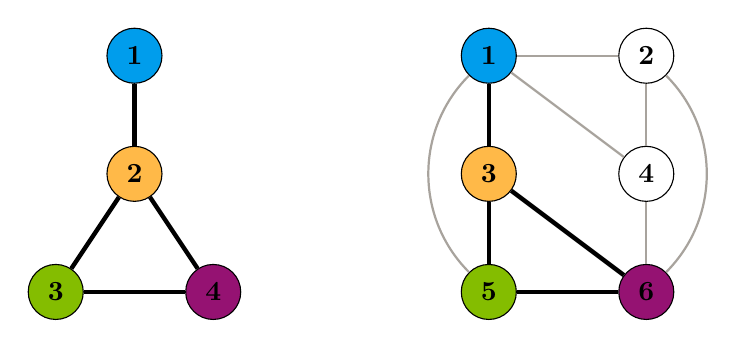
\begin{tikzpicture}
        \node[draw, circle, fill=uofgcobalt, inner sep=4pt, font=\bfseries] (Na) at (1,  0) {1};
        \node[draw, circle, fill=uofgpumpkin, inner sep=4pt, font=\bfseries] (Nb) at (1, -1.5) {2};
        \node[draw, circle, fill=uofglawn, inner sep=4pt, font=\bfseries] (Nc) at (0, -3) {3};
        \node[draw, circle, fill=uofgthistle, inner sep=4pt, font=\bfseries] (Nd) at (2, -3) {4};

        \draw [ultra thick] (Na) -- (Nb);
        \draw [ultra thick] (Nb) -- (Nc);
        \draw [ultra thick] (Nc) -- (Nd);
        \draw [ultra thick] (Nb) -- (Nd);

        \node[draw, circle, fill=uofgcobalt, inner sep=4pt, font=\bfseries] (N1) at (5.5,  0) {1};
        \node[draw, circle, fill=white, inner sep=4pt, font=\bfseries] (N2) at (7.5,  0) {2};
        \node[draw, circle, fill=uofgpumpkin, inner sep=4pt, font=\bfseries] (N3) at (5.5, -1.5) {3};
        \node[draw, circle, fill=white, inner sep=4pt, font=\bfseries] (N4) at (7.5, -1.5) {4};
        \node[draw, circle, fill=uofglawn, inner sep=4pt, font=\bfseries] (N5) at (5.5, -3) {5};
        \node[draw, circle, fill=uofgthistle, inner sep=4pt, font=\bfseries] (N6) at (7.5, -3) {6};

        \draw [thick, color=uofgsandstone!50] (N1) -- (N2);
        \draw [ultra thick] (N1) -- (N3);
        \draw [thick, color=uofgsandstone!50] (N1) -- (N4);
        \draw [thick, color=uofgsandstone!50] (N2) -- (N4);
        \draw [ultra thick] (N3) -- (N5);
        \draw [ultra thick] (N3) -- (N6);
        \draw [thick, color=uofgsandstone!50] (N4) -- (N6);
        \draw [ultra thick] (N5) -- (N6);
        \draw [thick, color=uofgsandstone!50] (N2) to [in=45, out=315] (N6);
        \draw [thick, color=uofgsandstone!50] (N1) to [in=135, out=225] (N5);
    \end{tikzpicture}\end{center}

\end{frame}

\begin{frame}{Induced Subgraph Isomorphism}

    \begin{center}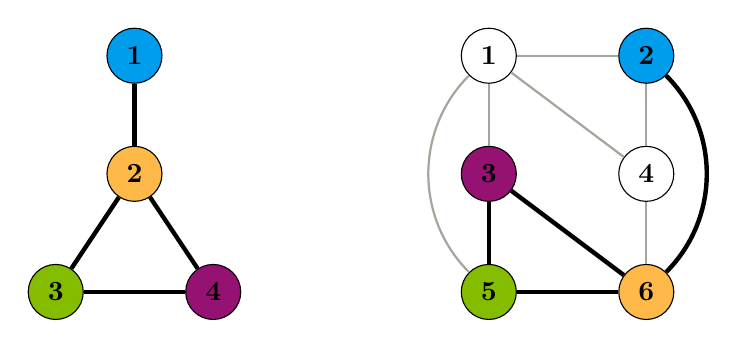
\begin{tikzpicture}
        \node[draw, circle, fill=uofgcobalt, inner sep=4pt, font=\bfseries] (Na) at (1,  0) {1};
        \node[draw, circle, fill=uofgpumpkin, inner sep=4pt, font=\bfseries] (Nb) at (1, -1.5) {2};
        \node[draw, circle, fill=uofglawn, inner sep=4pt, font=\bfseries] (Nc) at (0, -3) {3};
        \node[draw, circle, fill=uofgthistle, inner sep=4pt, font=\bfseries] (Nd) at (2, -3) {4};

        \draw [ultra thick] (Na) -- (Nb);
        \draw [ultra thick] (Nb) -- (Nc);
        \draw [ultra thick] (Nc) -- (Nd);
        \draw [ultra thick] (Nb) -- (Nd);

        \node[draw, circle, fill=white, inner sep=4pt, font=\bfseries] (N1) at (5.5,  0) {1};
        \node[draw, circle, fill=uofgcobalt, inner sep=4pt, font=\bfseries] (N2) at (7.5,  0) {2};
        \node[draw, circle, fill=uofgthistle, inner sep=4pt, font=\bfseries] (N3) at (5.5, -1.5) {3};
        \node[draw, circle, fill=white, inner sep=4pt, font=\bfseries] (N4) at (7.5, -1.5) {4};
        \node[draw, circle, fill=uofglawn, inner sep=4pt, font=\bfseries] (N5) at (5.5, -3) {5};
        \node[draw, circle, fill=uofgpumpkin, inner sep=4pt, font=\bfseries] (N6) at (7.5, -3) {6};

        \draw [thick, color=uofgsandstone!50] (N1) -- (N2);
        \draw [thick, color=uofgsandstone!50] (N1) -- (N3);
        \draw [thick, color=uofgsandstone!50] (N1) -- (N4);
        \draw [thick, color=uofgsandstone!50] (N2) -- (N4);
        \draw [ultra thick] (N3) -- (N5);
        \draw [ultra thick] (N3) -- (N6);
        \draw [thick, color=uofgsandstone!50] (N4) -- (N6);
        \draw [ultra thick] (N5) -- (N6);
        \draw [ultra thick] (N2) to [in=45, out=315] (N6);
        \draw [thick, color=uofgsandstone!50] (N1) to [in=135, out=225] (N5);

    \end{tikzpicture}\end{center}
\end{frame}

\begin{frame}{Benchmarking}

    \begin{itemize}
        \item Based upon chemical and computer vision datasets, we can handle patterns with 1,000
            vertices and targets with 10,000 vertices.
        \item Do these results reflect the worst case, or are they too optimistic?
        \item Can we create ``hard'' benchmark instances?
    \end{itemize}

\end{frame}

\begin{frame}{Randomly Selected Subgraphs}

    \begin{itemize}
        \item Start with a random target graph.
        \item Pick vertices at random to make a pattern.
        \item Shuffle the numbering.
        \item <2-> These instances will always be satisfiable!
    \end{itemize}

\end{frame}

\begin{frame}{Independently Random Subgraphs}

    \begin{itemize}
        \item Make a random target graph.
        \item Independently, make a random pattern graph.
        \item <2-> Will these instances ever be satisfiable?
    \end{itemize}

\end{frame}

\begin{frame}{A Phase Transition}
\end{frame}

\begin{frame}{2D Phase Transitions}
\end{frame}

\begin{frame}{3D Phase Transitions}
\end{frame}

\begin{frame}{Reductions}
\end{frame}

\begin{frame}[plain,noframenumbering]
    \begin{tikzpicture}[remember picture, overlay]
        \node at (current page.north west) {
            \begin{tikzpicture}[remember picture, overlay]
                \fill [fill=uofguniversityblue, anchor=north west] (0, 0) rectangle (\paperwidth, -1.7cm);
            \end{tikzpicture}
        };

        \node (logo) [anchor=north east, shift={(-0.3cm,-0.2cm)}] at (current page.north east) {
            \includegraphics*[keepaspectratio=true,scale=0.55]{UoG_keyline.pdf}
        };
    \end{tikzpicture}
\end{frame}

\end{document}

